\documentclass[tikz,border=6pt]{standalone}
\usepackage{ctex}
\usepackage{amsmath}
\usetikzlibrary{calc, arrows.meta}

\begin{document}
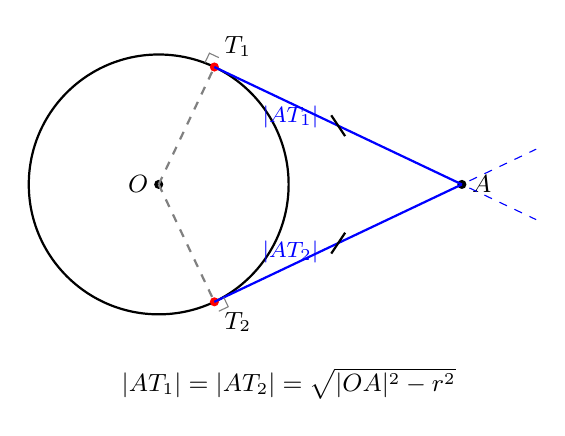
\begin{tikzpicture}[scale=1.1, thick]

% 圆外一点 A 引两条切线，切点 T1、T2

% 圆心 O 在原点，半径 r = 1.5
\coordinate (O) at (0, 0);
\def\r{1.5}

% 圆外一点 A
\coordinate (A) at (3.5, 0);

% 计算切点：|OA| = 3.5，切点在圆上，|OT| = r，|AT| = sqrt(|OA|^2 - r^2)
% 切点满足：OT ⊥ AT
% T1 和 T2 关于 OA 连线（x 轴）对称
% 设切点角度 theta = arccos(r / |OA|) = arccos(1.5/3.5) = arccos(3/7)
% cos(theta) = 3/7 ≈ 0.4286, sin(theta) = sqrt(1-(3/7)^2) = sqrt(40)/7 ≈ 0.9035
% T1 = (r*cos(theta), r*sin(theta)) = (1.5 * 3/7, 1.5 * sqrt(40)/7)
%    = (9/14, 1.5*sqrt(40)/7) ≈ (0.6429, 1.3553)
% T2 = (0.6429, -1.3553)

\coordinate (T1) at ({1.5*3/7}, {1.5*sqrt(40)/7});
\coordinate (T2) at ({1.5*3/7}, {-1.5*sqrt(40)/7});

% 画圆
\draw[black, thick] (O) circle [radius=\r];

% 圆心
\fill[black] (O) circle [radius=1.5pt];
\node[left, font=\small] at (O) {$O$};

% 外点 A
\fill[black] (A) circle [radius=1.5pt];
\node[right, font=\small] at (A) {$A$};

% 切点
\fill[red] (T1) circle [radius=1.5pt];
\node[above right, font=\small] at (T1) {$T_1$};

\fill[red] (T2) circle [radius=1.5pt];
\node[below right, font=\small] at (T2) {$T_2$};

% 两条切线 AT1, AT2
\draw[blue, thick] (A) -- (T1);
\draw[blue, thick] (A) -- (T2);

% 延伸切线少许（过 T1 往圆另一侧延长）
\draw[blue, dashed, thin] (T1) -- ($(A)!-0.3!(T1)$);
\draw[blue, dashed, thin] (T2) -- ($(A)!-0.3!(T2)$);

% 连 OT1, OT2（灰色虚线，表示半径⊥切线）
\draw[gray, dashed] (O) -- (T1);
\draw[gray, dashed] (O) -- (T2);

% 直角标记：OT1 ⊥ AT1
% 在 T1 处，OT1 方向 = T1 - O，AT1 方向 = T1 - A
% 直角小方块
\coordinate (odir1) at ($(\r,0)!(T1)!(O)$);  % 不直接用，下面手算
% OT1 单位向量：(T1 - O) / r = (3/7, sqrt(40)/7)
% AT1 单位向量：(T1 - A) / |AT1| = (0.6429-3.5, 1.3553) / sqrt((2.8571)^2+1.3553^2)
%   |AT1| = sqrt(3.5^2 - 1.5^2) = sqrt(12.25-2.25) = sqrt(10) ≈ 3.1623
%   单位向量 ≈ (-2.8571/3.1623, 1.3553/3.1623) = (-0.9035, 0.4286)
% 直角小方块边长 0.12
% 点 = T1 + 0.12*(OT1_unit) + 0.12*(AT1_unit)
\draw[gray, thin]
  ($(T1) + 0.12*({3/7}, {sqrt(40)/7})$)
  -- ($(T1) + 0.12*({3/7}, {sqrt(40)/7}) + 0.12*({-sqrt(40)/7}, {3/7})$)
  -- ($(T1) + 0.12*({-sqrt(40)/7}, {3/7})$);

% OT2 ⊥ AT2 的直角标记（T2 在 x 轴下方，y 坐标取负）
\draw[gray, thin]
  ($(T2) + 0.12*({3/7}, {-sqrt(40)/7})$)
  -- ($(T2) + 0.12*({3/7}, {-sqrt(40)/7}) + 0.12*({sqrt(40)/7}, {3/7})$)
  -- ($(T2) + 0.12*({sqrt(40)/7}, {3/7})$);

% 等长标记：|AT1| = |AT2|
% AT1 中点处标单撇
\coordinate (M1) at ($(A)!0.5!(T1)$);
\coordinate (M2) at ($(A)!0.5!(T2)$);

% 单撇（tickone 效果：手动画一短横线）
\draw[thick] ($(M1) + (-0.08, 0.12)$) -- ($(M1) + (0.08, -0.12)$);
\draw[thick] ($(M2) + (-0.08, -0.12)$) -- ($(M2) + (0.08, 0.12)$);

% 标注等长
\node[font=\footnotesize, blue] at ($(M1) + (-0.55, 0.1)$) {$|AT_1|$};
\node[font=\footnotesize, blue] at ($(M2) + (-0.55, -0.1)$) {$|AT_2|$};

% 说明等长
\node[font=\small, align=center] at (1.5, -2.3)
  {$|AT_1| = |AT_2| = \sqrt{|OA|^2 - r^2}$};

\end{tikzpicture}
\end{document}
